\section{Signal to Noise Ratio improvement}
\subsection{Convention and previous method}
\label{sec:previousmethod}
The  purpose  of this  section  is  to  investigate signal  processing
methods  to  increase the  detection  capability.\\  In the  following
section we  will only deal  with SNR.  We  won't deal with  the system
noise temperature,  at least not  directly, because it is  included in
the SNR.  All  of the following study is done in  a relative way, with
no need to set the noise temperature or the gain.  What we need to set
is  the  antenna/LNB  spectrum   (the  frequency  bandwidth)  and  the
electronics parameters  (cf section~\ref{sec:signalsim}).  \\The input
SNR  is defined  as  the ratio  of  the maximum  of  the signal  power
envelope over the  system noise average (not its  RMS).  However after
the detector, what  we want to compare is the  maximum signal with the
fluctuation of the  noise, so we will look at the  waveform in unit of
its fluctuation (  we will plot the ratio of  signal minus the average
noise over  the noise fluctuation).  We define $\rm SNR_{det}$  as the
maximum power  in unit of  noise fluctuation.\\To study the  effect of
filtering, we  use input signals with Gaussian  envelope.  Examples of
simulated traces are shown in the figure~\ref{fig:traceex}.
\begin{figure}[ht!]                                                             
  \centering                                                                    
  \hspace*{-3ex}                                                                
  \subfigure{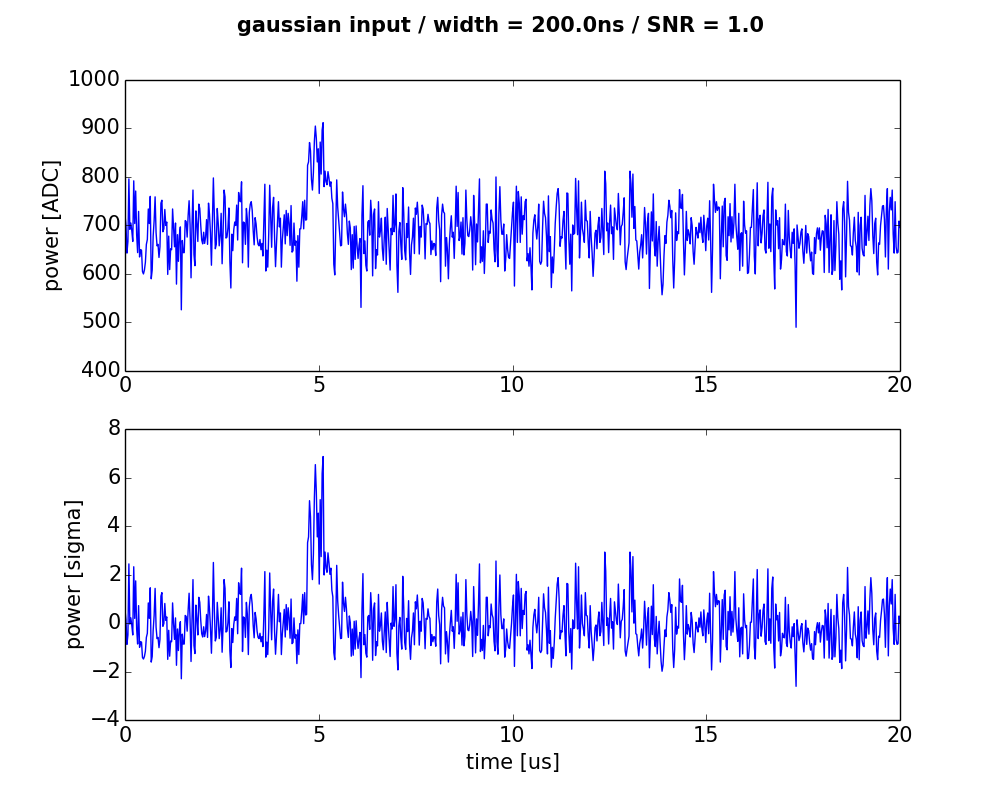
\includegraphics[width=0.49\linewidth]{ex1.png}}
  \subfigure{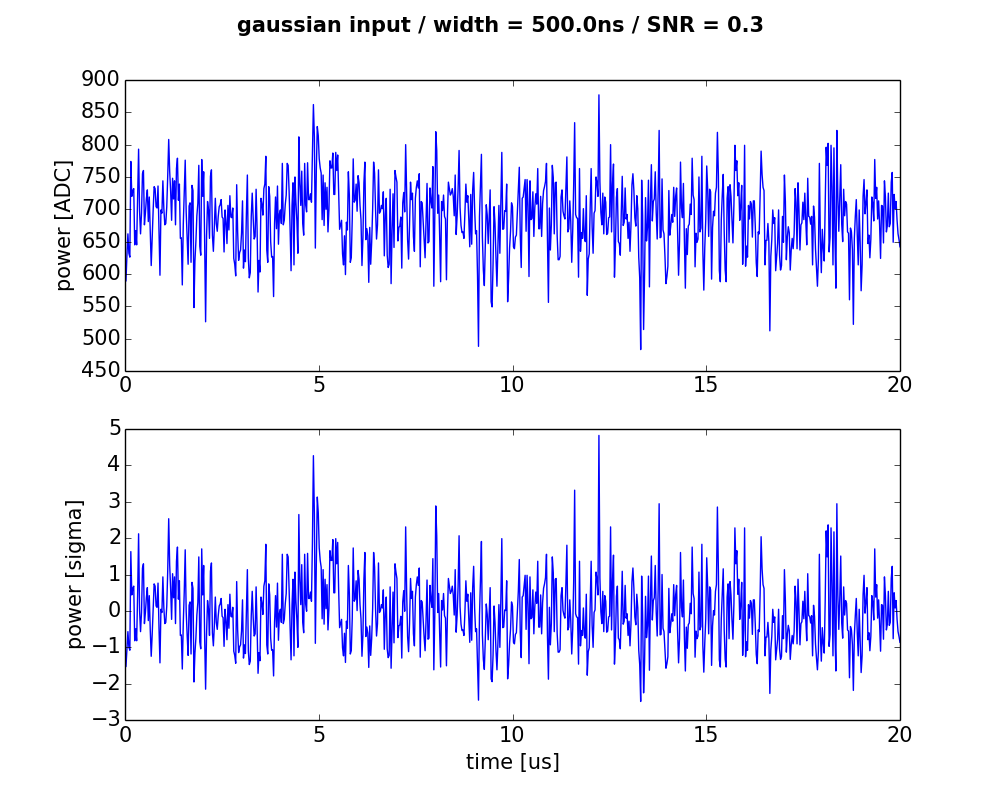
\includegraphics[width=0.49\linewidth]{ex2.png}}        
  \subfigure{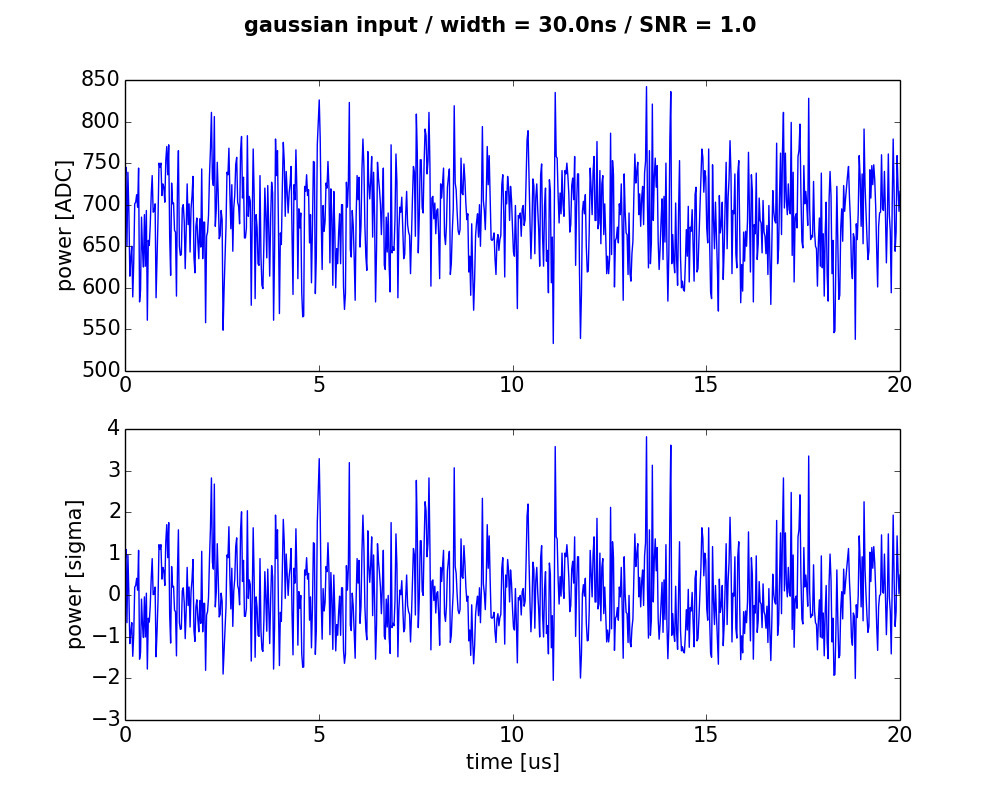
\includegraphics[width=0.49\linewidth]{ex3.png}}        
  \caption{three example of simulated trace with on top of each figure
    the signal in ADC counts, and on the bottom the signal in sigma}
  \label{fig:traceex}
\end{figure}
The signal  is clearly seen  when the width  of the gaussian  is large
enough, of a  few hundreds of ns, and  the SNR is of the  order of the
unity.  If  we decrease one of  these parameters we  start loosing the
signal into the noise.\\ The method implemented in \cite{mythesis} was
a simple peak search method. We would insure the background to be null
by setting a  high threshold (around 7 sigmas)  and asking the maximum
of the trace to be in a  window of \unit[4]{$\rm \mu s $}.  We can now
compute the  efficiency, that  is to say  the percentage  of simulated
event     that    would     pass    the     criteria,     with    this
method. Figure~\ref{fig:previousmethod} shows the detection efficiency
for such a peak search.
\begin{figure}[ht!]                                                             
  \centering                                                                    
  \hspace*{-3ex}                                                                
  \subfigure{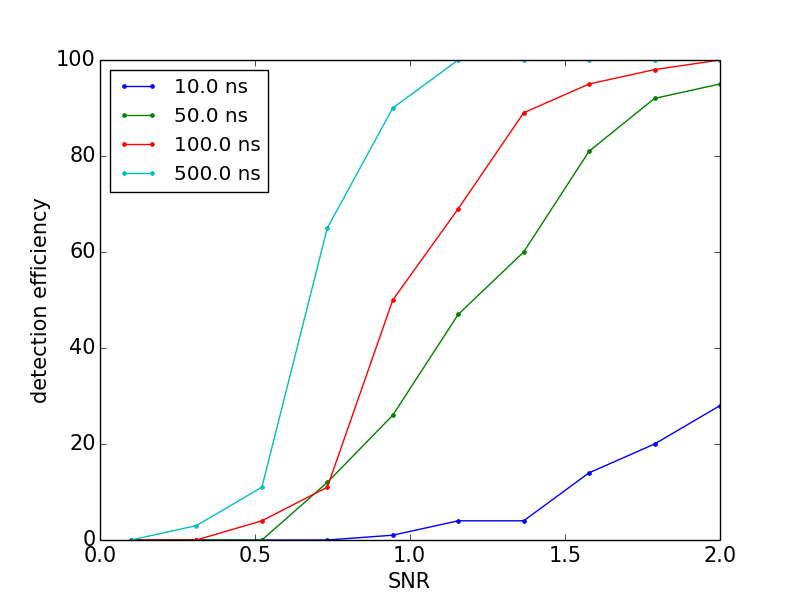
\includegraphics[width=0.49\linewidth]{efficiency.png}}
  \subfigure{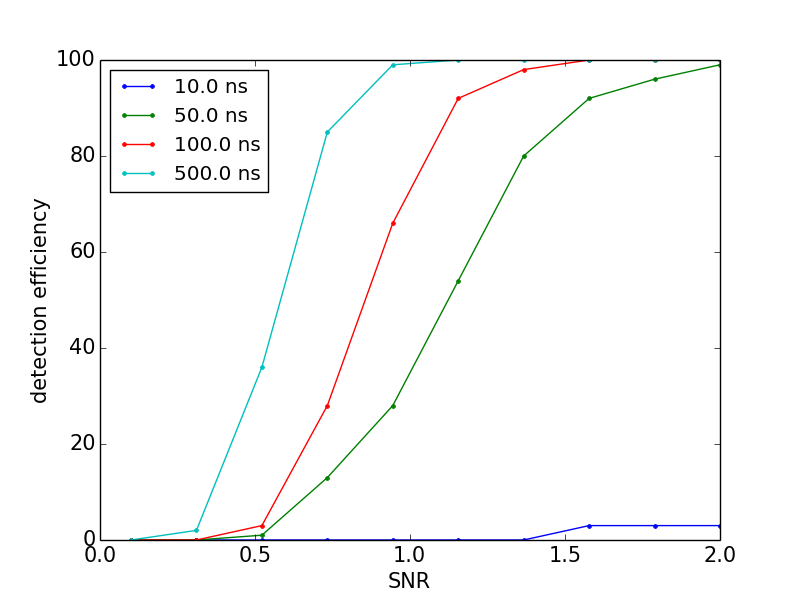
\includegraphics[width=0.49\linewidth]{efficiencygi.png}}        
  \caption{Detection  efficiency  with   peak  search  (left:  without
    capacitor, right: with capacitor)}
  \label{fig:previousmethod}
\end{figure}
\newpage
\subsection{Filtering}
The point of filtering is to  keep the signal and remove the noise. We
have simulated trace  with a large SNR and  produced their spectrum in
the  figure~\ref{fig:signalspectra}.   The shorter  the  signal ,  the
flatter the spectrum.   When the signal is too  short the spectrum has
no specific structure anymore so the filtering is useless. However, we
see that for the longer signal  we can filter out the high frequencies
and keep only the signal part at low frequency.
\begin{figure}[ht!]                                                             
  \centering                                                                    
  \hspace*{-3ex}                                                                
  \subfigure{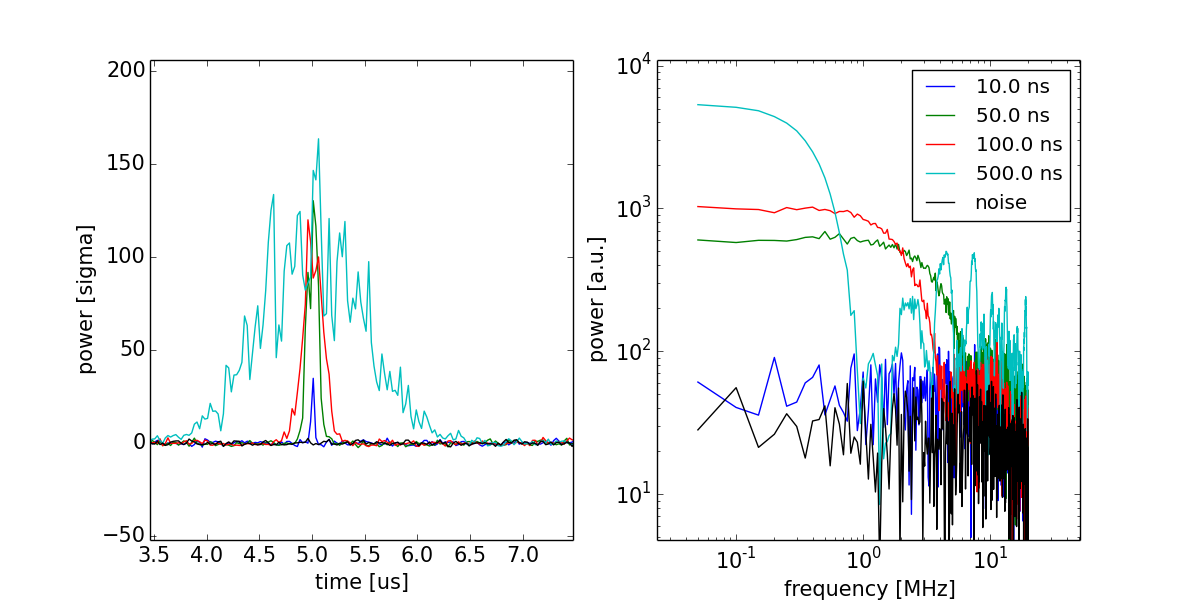
\includegraphics[width=0.8\linewidth]{signalspectra.png}}        
  \caption{spectra for various width of input and a SNR of 20.}
  \label{fig:signalspectra}
\end{figure}

\paragraph{low pass filter}
One method is to filter at  a given frequency.  From the spectra shown
in the figure~\ref{fig:signalspectra} we see that for a \unit[500]{ns}
signal  we  would   need  to  filter  with  a   cut  frequency  around
\unit[1]{MHz} and for  a \unit[50]{ns} long signal a  cut frequency of
\unit[10]{MHz}.  We  apply these filter to simulated  traces, and then
convert  the trace  in sigma  units, some  examples are  shown  in the
figure~\ref{fig:exfilter}.  We  can improve the signal  to noise ratio
$\rm SNR_{det}$ when  the correct filter ( matching  the signal...) is
chosen: low cut frequency for  long signals and high cut frequency for
short signals.

\begin{figure}[ht!]                                                             
  \centering                                                                    
  \hspace*{-3ex}                                                                
  \subfigure{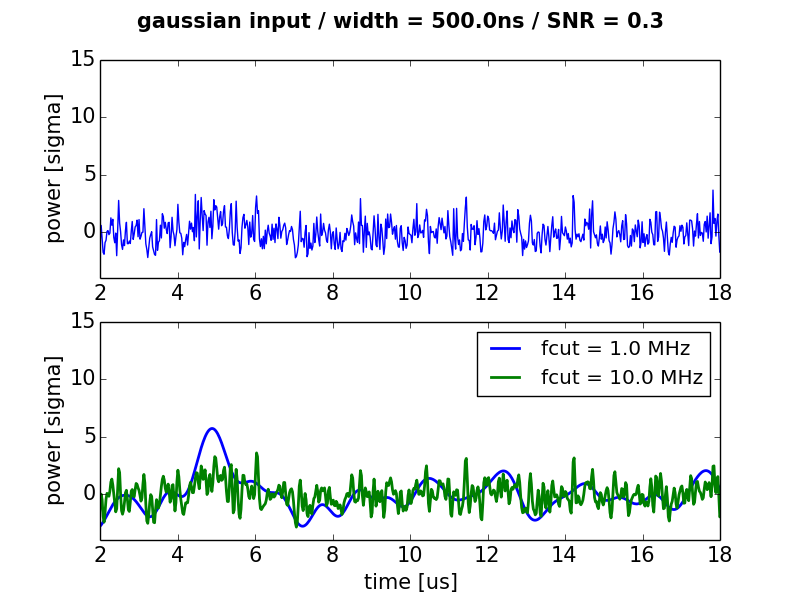
\includegraphics[width=0.49\linewidth]{exfilter.png}}        
  \subfigure{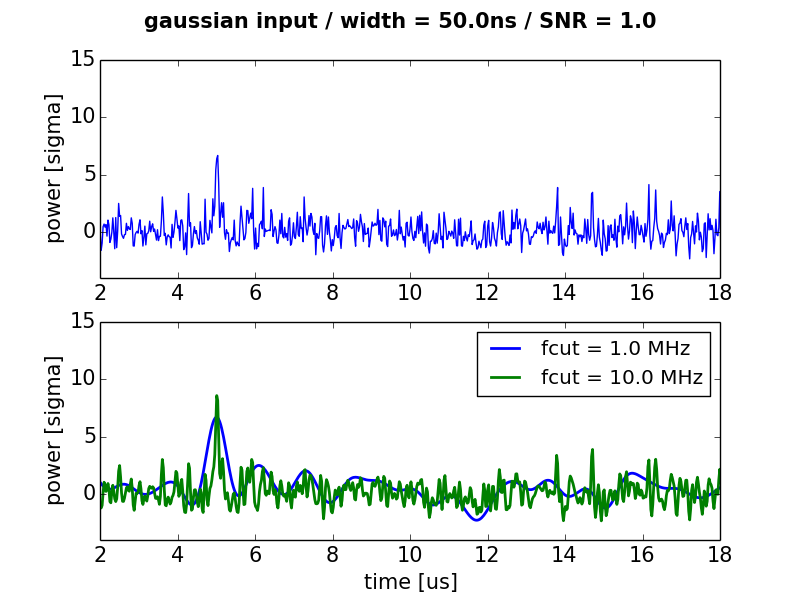
\includegraphics[width=0.49\linewidth]{exfilter2.png}}        
  \caption{Examples of  filtered trace with low pass  filter. The best
    filter depends on the input signal.}
  \label{fig:exfilter}
\end{figure}


\paragraph{matched filter}
The best way  to find a known signal into a  measured (noise + signal)
waveform is to cross correlate the measured waveform with the expected
signal itself.  It is equivalent to filter it with the expected signal
spectrum.   (in  principle  you  also  want to  weight  your  filter's
coefficient with the noise spectrum but in our case the noise spectrum
is really  flat so the  improvement won't be important).   The matched
filter is  a very effective technique  when the signal  has a distinct
signature in the frequency spectrum. In our case, the expected signals
are rather  simple, and the matched  filter will look like  a low pass
filter. But  by applying  the matched  filter we are  sure to  use the
right filter, see  for instance in the figure~\ref{fig:exmatched}.\\We
can   now   compute   the   detection   efficiency,   shown   in   the
figure~\ref{fig:efficiencymatched}, using  the same parameters  than in
section~\ref{sec:previousmethod}.
\begin{figure}[ht!]                                                             
  \centering                                                                    
  \hspace*{-3ex}                                                                
  \subfigure{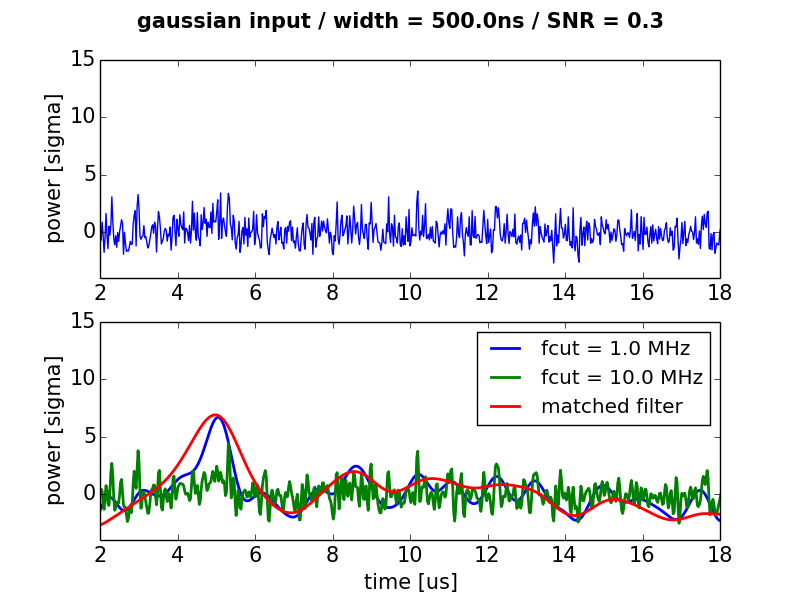
\includegraphics[width=0.49\linewidth]{exmatched.png}}        
  \subfigure{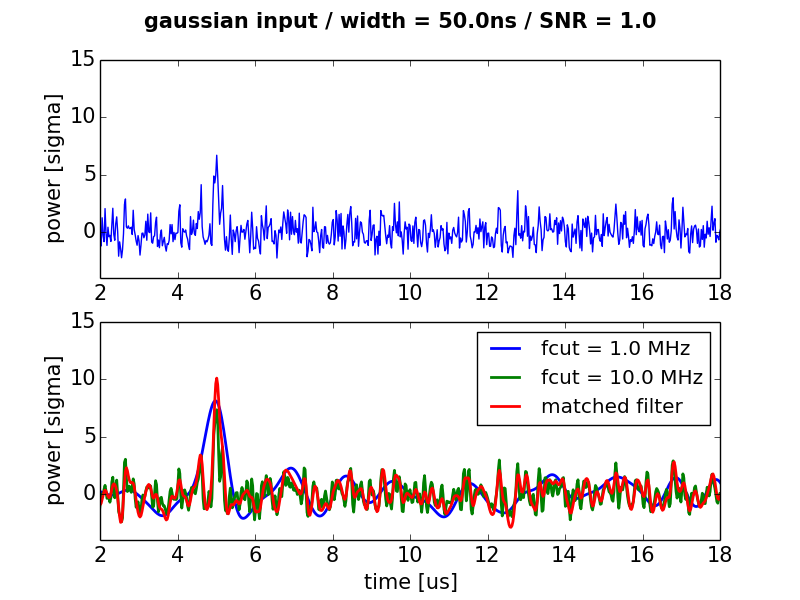
\includegraphics[width=0.49\linewidth]{exmatched2.png}}        
  \caption{Examples of filtered trace with low pass filter and matched
    filter.  In   both  cases  the  matched  filter   gives  the  best
    $SNR_{det}$}
  \label{fig:exmatched}
\end{figure}
\begin{figure}[ht!]                                                             
  \centering                                                                    
  \hspace*{-3ex}                                                                
  \subfigure{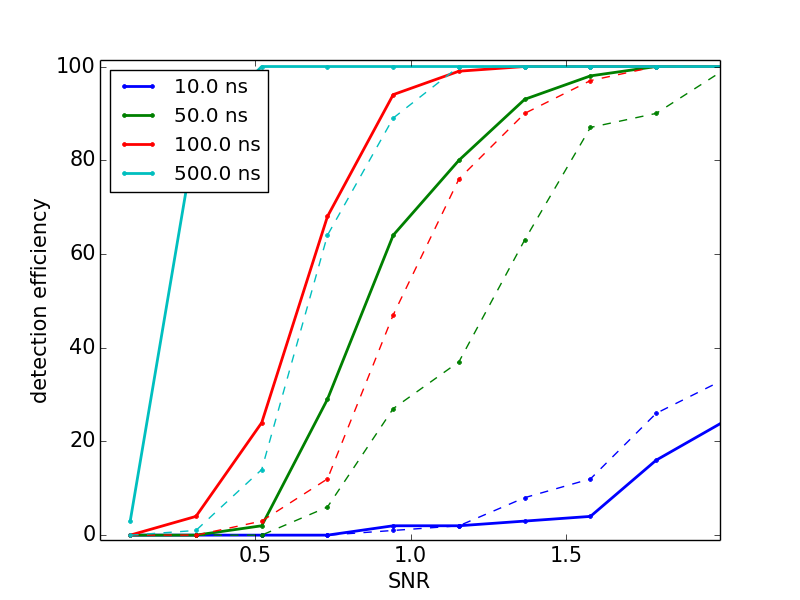
\includegraphics[width=0.49\linewidth]{efficiencymatched.png}}        
  \subfigure{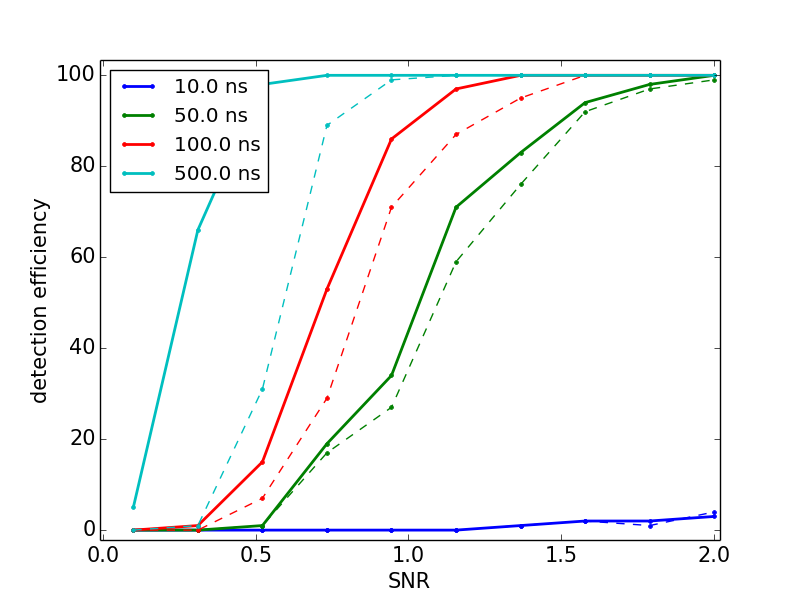
\includegraphics[width=0.49\linewidth]{efficiencymatchedgi.png}}        
  \caption{Detection efficiency after the matched filter processing in
    solid line.  The dashed line represents the  results found without
    filtering.}
  \label{fig:efficiencymatched}
\end{figure}

The largest improvement is  obtained for long signals, \unit[500]{ns},
for which  we reach 100\%  efficiency for an  input SNR of  around 0.5
instead of 1 when no processing filter is applied. For shorter signals
the improvement is clear especially when no capacitor is present after
the power detector  (figure~\ref{fig:efficiencymatched} left).  When the
capacitor is present, the  signal is already filtered analogically and
the numerical filter that we apply has less effect.
